\documentclass[pre,amssymb,showpacs,showkeys,preprint]{revtex4}
\usepackage[T1]{fontenc}
\RequirePackage{times}
\usepackage{graphicx}
\newtheorem{prop}{Proposition}
\begin{document}
%\sloppy



\title{Scale-Invariant Cellular Automata}

\author{Martin Schaller}
\email{martin_schaller@acm.org}
\affiliation{Oesterreichische Nationalbank,
Otto-Wagner-Platz 3, 1090  Vienna, Austria}

\author{Karl Svozil}
\email{svozil@tuwien.ac.at}
\homepage{http://tph.tuwien.ac.at/~svozil}
\affiliation{Institut f\"ur Theoretische Physik, University of Technology Vienna,
Wiedner Hauptstra\ss e 8-10/136, A-1040 Vienna, Austria}




\begin{abstract}
A new kind of scale-invariant cellular automaton is introduced which is based on recursively nested
lattices embedded in Euclidean space.
This new computational model is inherently scale-invariant, opening the way to the broader concept
of scale-invariant computing and evolution.
This model is capable of solving decision problems such as the
halting problem by allowing the construction of accelerated Turing machines.
\end{abstract}


\pacs{05.90.+m,02.90.+p,47.54.-r}
\keywords{Cellular Automata, pattern formation}


\maketitle

\section{Introduction}
%Cellular automata are defined on a regular lattice.
%Mapping this lattice to Euclidean space introduces a natural unit of length, the distance
%between two adjacent cells.
%We extend the cellular automaton model by nesting an infinite number of lattices recursively.
%Choosing an appropriate timing behavior, we are able to achieve a constant speed of information
%propagation throughout the nested lattices.
%To our knowledge, this is the first computational model, which is scale invariant.
%We show that, due to the scale invariance and the constant information propagation speed, this new
%computational model has hypercomputing capabilities, i.e. is capable to solve Turing's Halting
%problem.

Every physically relevant computational model must be mapped into space-time and {\it vice versa.}
In this line of thought, Von Neumann's self-reproducing Cellular Automata \cite{v-neumann-66}
have been envisioned by Zuse \cite{zuse-67,zuse-69,zuse-94,zuse-70}
and other researchers  \cite{fredkin,toffoli-margolus-90,wolfram-2002}
as  ``calculating space;''
i.e., as a
locally connected grid of finite automata \cite{hopcroft}
capable of universal algorithmic tasks, in which
observers are embedded \cite{toffoli:79}.
This model is conceptually discreet and
noncontinuous and resolves the eleatic ``arrow''
antinomy \cite{zeno,ki-57,gruenbaum:68,sv-aut-rev}
against motion in discrete space by introducing
the concept of information about the state of motion in between time steps.

In contrast to the assumption of a tesselation of
configuration space, there is no direct
physical evidence supporting such an assumption.
On the contrary, given enough energy, physical configuration space seems
to be divisible potentially without any limits.
An expression for this property is the Zeno
oracle \cite{weyl:49} capable of hypercomputation
proposed
in the relativistic context
\cite{thom:54,benna:62,pit:90,ear-nor:93,hogarth1,hogarth2,beth-59,le-91}.
Davies \cite{davies-01} describes in some detail how to build an infinite computing machine within
a continuous Newtonian universe, thereby also requiring that space-time is infinitely divisible and
discusses the physical and philosophical
implications.

The following model unifies the conceptional clarity of
von Neumann's Cellular Automaton model with the
requirement of infinite divisibility of cell space.

\section{Scale-Invariant Cellular Automata}

\emph{Cellular automata} are dynamical systems in which space and time are discreet.
The states of cells in a regular lattice are updated synchronously according to a local deterministic
interaction rule.
The rule gives the new state of each cell as a function of the old states of some nearby states,
it neighbors.
Each cell obeys the same rule, and has a finite (usually small) number of states.
For a more comprehensive introduction to cellular automata, we refer to
\cite{wolfram-86, gutowitz, ilachinski01}.

A \emph{scale-invariant cellular automaton} (SCA) operates like an ordinary
\emph{cellular automaton} (CA) on a cellular space, consisting of a regular arrangement of cells,
whereby each cell can hold a value out of a set of discrete states.
Whereas the cellular space of a CA consists of a regular one- or higher
dimensional lattice, a SCA operates on a cellular space of recursively nested lattices.
As by ordinary CAs, the cellular space of a SCA can be embedded in Euclidean space.
The assumption of a maximum speed of information propagation,
called in the following \emph{speed of light}, of the embedded cellular space, is used to derive the
timing behavior of the SCA model.
The SCA time behavior differs from the time behavior of CA in so far,
as cells in the same lattice synchronously change their state \cite{Morelli_Zanette}, but
as cells are getting smaller in deeper nested lattices, the time steps between state changes in
the same lattice decreases and approaches 0 in the limit.
The SCA model gains its extraordinary computing capabilities by introducing a local rule that
allows for interaction between adjacent lattices \cite{BoFeng_MengDing}.
We will introduce the SCA model for the one-dimensional case, the extension to higher dimensions
\cite{Brunnet_Chate} is
straightforward.

\subsection{Space Structure}

Let $L_0$ be an one-dimensional lattice, where cells are indexed by integers $i \in \mathbb Z$.
This lattice is mapped to intervals of real numbers in a natural way, by mapping cell $i$ to the
half-open interval $[i, i+1) \subset \mathbb R$, whereby the center of cell $i$ is located at
$i + \frac{1}{2}$.
There is a one-to-one correspondence between cells and intervals of the form
$[i, i+1)$, where $i \in \mathbb Z$, which allows us to identify cells with their corresponding
intervals.
Splitting each cell into two subcells of equal size leads to the next finer lattice $L_{-1}$, where
cell $i, i \in \mathbb Z$, is mapped to the interval $[\frac{i}{2}, \frac{i+1}{2})$.
We call $L_0$ the superlattice of $L_{-1}$ and $L_{-1}$ the sublattice of $L_0$.
In general, we define the lattice $L_k$, $k \in \mathbb Z$, as the set of cells $[2^ki, 2^k(i+1))$,
$i \in \mathbb Z$.
The cellular space of a scale-invariant cellular automaton is formed by the union of all cells of
all lattices $L_k$, $k \in \mathbb Z$.

Let $c$ be a cell of lattice $L_k$ with index $i$, identified by the interval $[2^ki, 2^k(i+1))$.
We call cell $c^\prime$ of lattice $L_{k+1}$ with index $\lfloor \frac{i}{2} \rfloor$ and interval
$[2^{k+1}\lfloor \frac{i}{2} \rfloor, 2^{k+1}(\lfloor \frac{i}{2} \rfloor+1))$ \emph{parent cell}
of $c$ and we call $c$ \emph{child cell} of $c^\prime$.
Obviously, each cell has one parent cell and two children cells.
Transferring the ordering of the real numbers to the cells, we can speak of a left or right
child.
We introduce two predicates $\emph{left}$ and $\emph{right}$ to denote the relative position of a
cell relative to its parent cell:
$\mbox{left}(c) = \mbox{true}$ if and only if $c$ is the left child cell of its parent cell.
Analogously, we define the predicate $\mbox{right}(c)$.
Of course $\mbox{left}(c) = \neg \mbox{right}(c)$ holds.

A cell within a lattice $L_k$ shall be connected to its left and right neighbor, which basically
forms the topological structure of an ordinary CA.
To allow for interaction between adjacent cells, we additionally link a cell with its parent cell
and its two children cells.
Cell $i$ of lattice $L_k$ is therefore connected to
\begin{enumerate}
\item its left neighbor cell $i-1$ and to its right neighbor cell $i+1$ of the same lattice $L_k$;
\item to its parent cell $\lfloor \frac{i}{2} \rfloor$ in the superlattice $L_{k+1}$; and
\item to the left child cell $2i$ and to the right child cell $2i+1$ in the sublattice $L_{k-1}$.
\end{enumerate}
Fig.~\ref{fig:1-dim-interaction} depicts the space and
topological structure of the cellular space, which is inherently scale-invariant.
Please note, that the separation of the lattices in the figure serves only as visual aid, the
cellular space is strictly one-dimensional.

Let $c$ be a cell in the cellular space.
For easier reference, we introduce the following neighborhood operators to refer to the neighbors
of a cell $c$.
\begin{enumerate}
\item $c_{\leftarrow}$ denotes the left neighbor, $c_{\rightarrow}$ the right neighbor of $c$ in
the same lattice;
\item $c_{\uparrow}$ denotes the parent cell in the superlattice; and
\item $c_{\swarrow}$ denotes the left child cell, $c_{\searrow}$ denotes the right child cell
in the sublattice.
\end{enumerate}

Let $c_1$ be a cell in the cellular space, represented by the interval $[a_1, b_1)$.
We define the length of the cell $c_1$ as the length of the interval, which is $b_1 - a_1$.
Let $c_2$ be a further cell, represented by
the interval $[a_2, b_2)$.
We define the distance $d$ between the cells $c_1$ and $c_2$ as the distance of their center points:
$d(c_1, c_2) = |\frac{b_2 - a_2}{2} - \frac{b_1 - a_1}{2}|$.
The distance $d$ forms a metric on the set of intervals in the cellular space.

\begin{figure}
\begin{center}
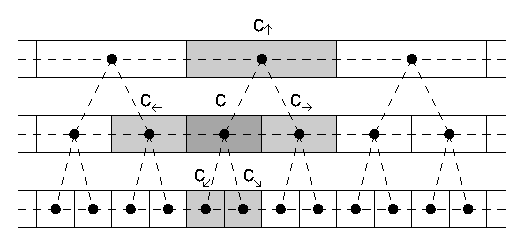
\includegraphics{2006-sica-OneDimInteraction2.eps}
\caption{\label{fig:1-dim-interaction} Space and topological structure of a SCA.}
\end{center}
\end{figure}

%\begin{figure}
%\begin{center}
%%\scalebox{1}[1]{\includegraphics[0,0][500,500]{2006-sica-TwoDimLattice.png}}
%\includegraphics{2006-sica-TwoDimPartition.eps}
%\caption{\label{fig:2-dim-grid} Nested two-dimensional lattices}
%\end{center}
%\end{figure}

\subsection{Time Behavior}

The embedding of the cellular space in Euclidean space,
which is for the one-dimensional case just the real numbers $\mathbb R$,
and the assumption of a maximum speed
of information propagation in the cellular space, the speed of light of the SCA, is used to
determine the time behavior of the SCA.
Without loss of generality, we set the speed of light in the cellular space to 1.
That is, a signal can travel a distance $x$ in time $x$.

We consider a lattice $L_k$ of the cellular space, and let us lead by the time behavior of
ordinary CAs.
All cells in the lattice shall synchronously change state, and all time steps between state changes
shall be of the same length.
As far as cells in the same lattice are concerned, a state change of cell $c$ shall depend on
the former state of $c$ and on the former states of its
both neighbors $c_\leftarrow$ and $c_\rightarrow$.
Since the length of a cell in lattice $L_k$ is $2^k$, a state change of a cell needs at least
the time $2^k$ to propagate to its neighbor.
We set the length of a time step in lattice $L_k$ therefore to this optimum value $2^k$.
Therefore, the length of a time step is identical to the Euclidean length of the cell, with the
implication, that a cell performs two state changes in the time its parent cell performs one state
change.

\begin{figure}
\begin{center}
\scalebox{0.2}{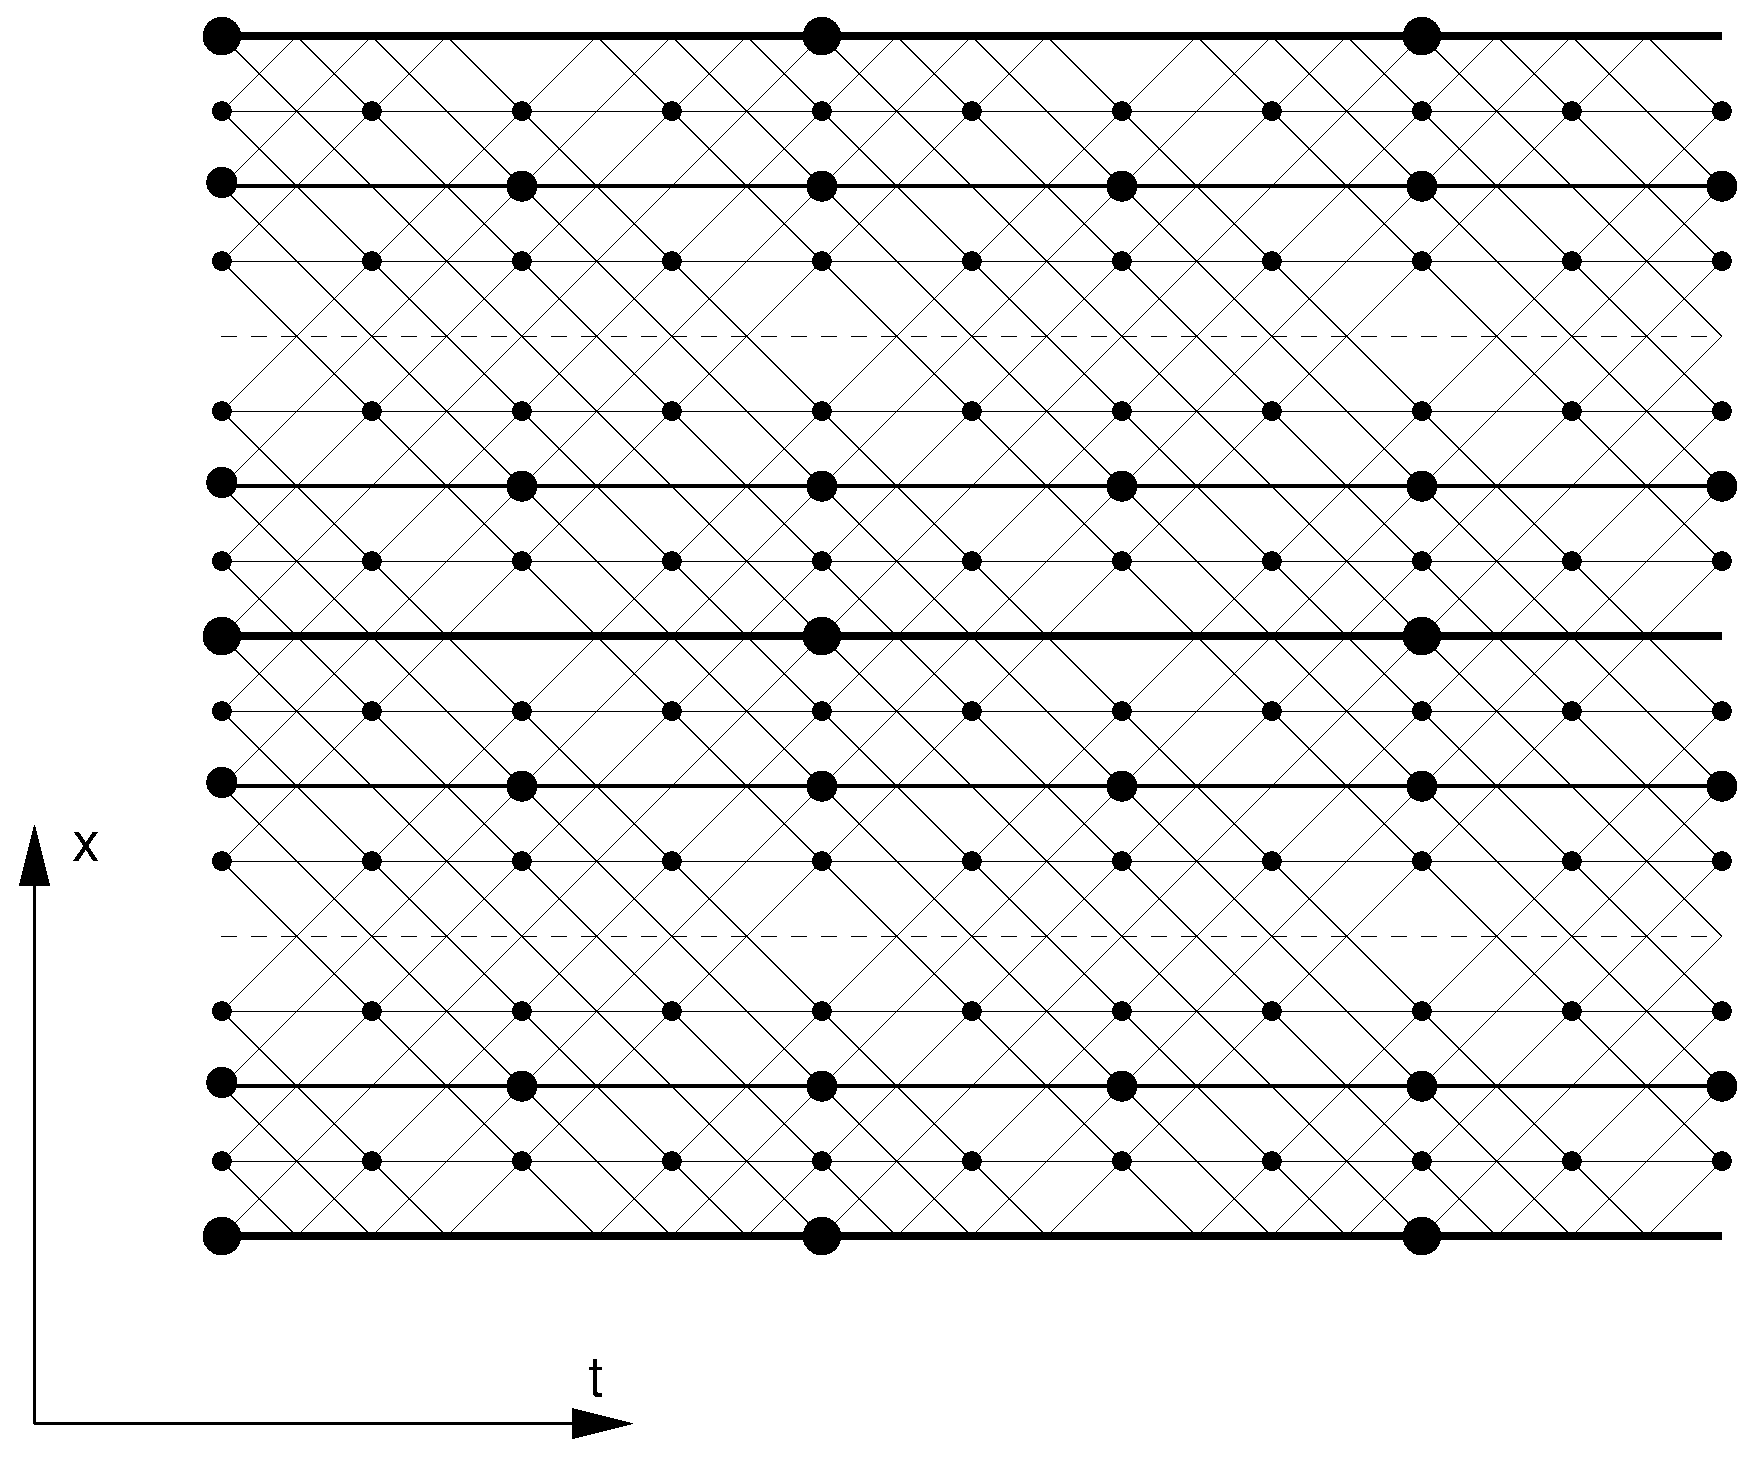
\includegraphics{2006-sica-SpaceTime2.eps}}
\caption{\label{fig:synchronous-space-time} Space-Time diagram of a synchronous SCA.}
\end{center}
\end{figure}

\begin{figure}
\begin{center}
\scalebox{0.2}{\includegraphics{2006-sica-SpaceTime.eps}}
\caption{\label{fig:asynchronous-space-time} Space-Time diagram of an asynchronous SCA.}
\end{center}
\end{figure}

\begin{figure}
\begin{center}
\scalebox{0.5}{\includegraphics{2006-sica-SynSCATimeBehavior.eps}}
\caption{\label{fig:synchronous-time} Time diagram of a synchronous SCA.}
\end{center}
\end{figure}

\begin{figure}
\begin{center}
\scalebox{0.5}{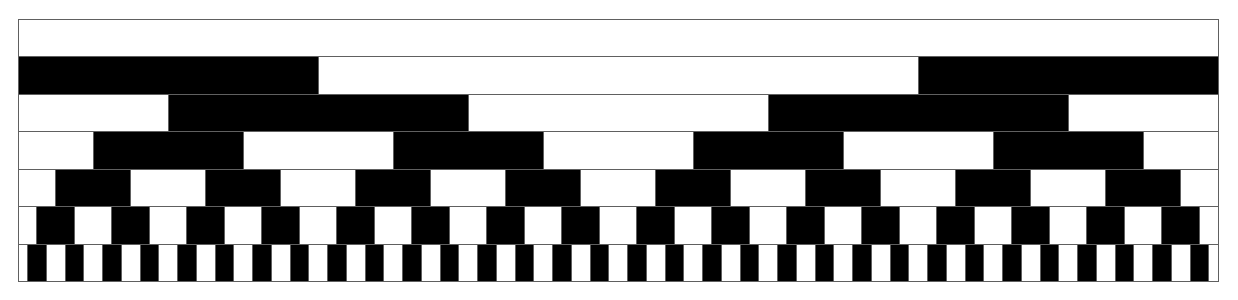
\includegraphics{2006-sica-AsynSCATimeBehavior.eps}}
\caption{\label{fig:asynchronous-time} Time diagram of an asynchronous SCA.}
\end{center}
\end{figure}

Even if the length of a time step per lattice is fixed, there is still the possibility
of a time lag (or offset) between state changes in adjacent lattices.
Fig.~\ref{fig:synchronous-space-time} and Fig.~\ref{fig:asynchronous-space-time} depict
the space-time diagrams of two SCAs with different offsets.
The points mark the center of cells, larger points indicates cells in coarser lattices.
The figures illustrates the information flow for three adjacent lattices.
The two diagonal outgoing lines of a point correspond to a signal propagation with the
speed of light.

Fig.~\ref{fig:synchronous-space-time} illustrates the time-space behavior of a SCA,
where a cell synchronously changes state with every second time step of its children cells.
The temporal behavior of this automaton is depicted in Fig.~\ref{fig:synchronous-time}.
State changes of cells occur at the horizontal transition from a white interval to a black one
or vice versa.
The transition from a black interval to a white one is synchronous with the state change of the
parent cell, the transition from a white interval to the black one is asynchronous.
We call a SCA featuring this this temporal behavior \emph{synchronous}.

The time steps in the evolution of an ordinary CA can be enumerated by integers.
For SCAs, we choose another enumeration schema.
In the most general form, one might specify the time of a state change
in a SCA as a series of binary
numbers: $(b_i)_{i \in \mathbb{Z}}$; $b_i \in \{0,1\}$.
The $n$-th digit shall be 1 if the last state change in layer $n$ was asynchronous
(black-colored time interval), and $0$ if the state change was synchronous
(white-colored time interval).
If we are only interested in a certain space-time region of the CA, only including cells in a
certain range of lattices, it is sufficient to specify a finite binary number
$(b_k, b_{k+1}, \ldots, b_l)$.
Using the convention, the state changes in Fig.~\ref{fig:synchronous-time} occur at
time $(0,0,0,0,0,0,0), (0,0,0,0,0,0,1), \ldots, (0,1,1,1,1,1,1)$.

Fig.~\ref{fig:asynchronous-space-time} illustrates a SCA with a
different temporal behavior than the former one.
This automaton is more efficient with regard to the information propagation to the neighbor lattices,
because the affected state changes lay on the edge of the light cone of the source state change.
All state changes occur asynchronously to state changes in other layers.
Therefore, we call this class of SCAs \emph{asynchronous}.
The temporal behavior of this kind of automata is depicted in Fig.~\ref{fig:asynchronous-time}.

By formulating the local rule, we have to refer to the past state changes of the neighborhood cells.
Similiarly to the neighborhood operators, we introduce time operators that given the time of
state change of a specified cell, map this time to the times of state changes in the past either
in the same layer or the adjacent ones.
Let $t$ be the time of a state change of a cell $c$ in lattice $L_k$.
\begin{enumerate}
\item $t_\leftarrow$ denotes the time of the last state change of $c$ before $t$;
\item $t_\uparrow$ denotes the time of the last state change of the parent cell $c_\uparrow$ before
 $t$;
\item $t_\searrow$ denotes the last state change of its child cells $c_\swarrow,$ and $c_\searrow$
before $t$;
\item $t_\swarrow$ denotes the second last state of its child cells $c_\swarrow,$ and $c_\searrow$
before $t$.
\end{enumerate}

Furthermore, we introduce two predicates, to distinguish whether a state change of a cell $c$ is the
first one or the second one after the state change of its parent cell $c_\uparrow$.
Let $t$ be the time of a state change of a given cell $c$:
$\mbox{first}(t) = \mbox{true}$, if and only if $t$ is the time of the first state change after
$t_\uparrow$.
Analogously, we define $\mbox{second}(t)$.
Since in a synchronous SCA several lattices might change state at the same time, we have to
specify the lattice where the state change occurs, if the lattice is not implicitly given.

Fig.~\ref{fig:1-dim-state-changes} depicts the temporal dependencies of two state changes at time
$t$ and $t^\prime$ for an
asynchronous SCA.

\subsection{Local Rule}

Knowing the space structure and the temporal behavior of the SCA model,
we can now consider the interaction and dependencies of state changes in adjacent cells,
which give this kind of automata its powerful computing capabilities.

Each cell of the SCA is in a certain state, out of the discrete state set $Z$.
We express the local rule of a SCA as a set of four local functions.
At each time step exactly one of these functions is applied to determine the new state of a cell,
depending on the relative position of a cell to its parent cell and of the time relative to
the time of the last state change of the parent cell.
We denote the state of a cell $c$ at time $t$ by $s(c,t)$.
The local rule is then given by
\[
s(c,t) = \left\{
\begin{array}{l}
f_{L1}(
	s(c_\uparrow, t_\uparrow),
	s(c_\leftarrow, t_\leftarrow), s(c, t_\leftarrow), s(c_\rightarrow, t_\leftarrow),
	s(c_\swarrow, t_\swarrow), s(c_\searrow, t_\swarrow),
	s(c_\swarrow, t_\searrow), s(c_\searrow, t_\searrow)
)
\\
\hspace{0.3in} \mbox{if left$(c)$ and first$(t)$;} \vspace{0.1in}
\\
f_{L2}(
	s(c_\uparrow, t_\uparrow),
	s(c_\leftarrow, t_\leftarrow), s(c, t_\leftarrow), s(c_\rightarrow, t_\leftarrow),
	s(c_\swarrow, t_\swarrow), s(c_\searrow, t_\swarrow),
	s(c_\swarrow, t_\searrow), s(c_\searrow, t_\searrow)
)
\\
\hspace{0.3in} \mbox{if left$(c)$ and second$(t);$}  \vspace{0.1in}
\\
f_{R1}(
	s(c_\uparrow, t_\uparrow),
	s(c_\leftarrow, t_\leftarrow), s(c, t_\leftarrow), s(c_\rightarrow, t_\leftarrow),
	s(c_\swarrow, t_\swarrow), s(c_\searrow, t_\swarrow),
	s(c_\swarrow, t_\searrow), s(c_\searrow, t_\searrow)
)
\\
\hspace{0.3in} \mbox{if right$(c)$ and first$(t)$;} \vspace{0.1in}
\\
f_{R2}(
	s(c_\uparrow, t_\uparrow),
	s(c_\leftarrow, t_\leftarrow), s(c, t_\leftarrow), s(c_\rightarrow, t_\leftarrow),
	s(c_\swarrow, t_\swarrow), s(c_\searrow, t_\swarrow),
	s(c_\swarrow, t_\searrow), s(c_\searrow, t_\searrow)
)
\\
\hspace{0.3in} \mbox{if right$(c)$ and second$(t).$} \\

\end{array}
\right.
\]

\begin{figure}
\begin{center}
\scalebox{0.7}{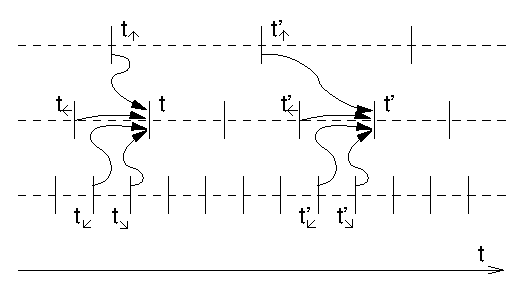
\includegraphics{2006-sica-StateChanges2.eps}}
\caption{\label{fig:1-dim-state-changes} Temporal dependencies of state changes of an an
asynchronous SCA at time $t$ and $t^\prime$.}
\end{center}
\end{figure}

We denote a SCA by the tuple $A = (Z, f_{L1}, f_{L2}, f_{R1}, f_{R2})$.
We remark that the SCA model is truly an extension of the CA model, because it includes the CA model
as a special case, since the definition of the local rule of the
SCA includes the possibility of a local rule of the form
$f(s(c_\leftarrow, t_\leftarrow), s(c, t_\leftarrow), s(c_\rightarrow, t_\leftarrow))$,
which is the constituting rule of a one-dimensional 3-neighborhood CA.

The local rules given above are very general and include, for example, the set of rules that either
do not depend on $t_\swarrow$ or on $t_\searrow$.
In Section \ref{sec-sim-tm-with-sca} we will see that the temporal dependency on
$t_\searrow$ introduces some subtleties and that the evolution of the SCA is only then guaranteed,
if one introduces the so called \emph{short-circuit rule evaluation}.

\subsection{Scale-Invariant Cellular Branch Automata}
\label{sec-sim-tm-with-sca}

In this section, we investigate a subclass of the one-dimensional SCAs.
Pick a cell from an one-dimensional SCA, together with all its direct and indirect children.
These cells form a tree-like structure, where siblings at the same level are connected,
see Fig.~\ref{fig:linear-sub-ca}.
If we choose the local rule in such a way, that the evolution of a cell is independent from its
siblings and from its right child cell, the cells that are dependent on each other form a branch of the tree,
depicted in the figure inside the dashed line.

\begin{figure}
\begin{center}
\scalebox{0.7}{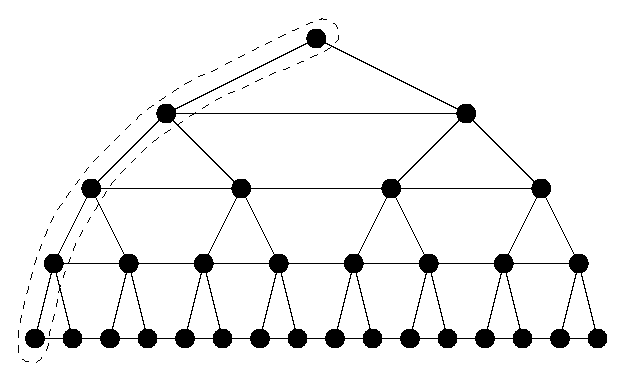
\includegraphics{2006-sica-LinearConnection.eps}}
\caption{\label{fig:linear-sub-ca} Connection graph of a scale-invariant cellular automata.}
\end{center}
\end{figure}

If we remove the dependencies to the other cells, the local rule takes on the following form:
\[
s(c,t) = \left\{
\begin{array}{l}
f_{1}(
	s(c_\uparrow, t_\uparrow),
	s(c, t_\leftarrow),
	s(c_\swarrow, t_\swarrow),
	s(c_\swarrow, t_\searrow)
) \mbox{  if first$(t)$;} \\
f_{2}(
	s(c_\uparrow, t_\uparrow),
	s(c, t_\leftarrow),
	s(c_\swarrow, t_\swarrow),
	s(c_\swarrow, t_\searrow)
) \mbox{  if second$(t)$.} \\
\end{array}
\right.
\]

We call this kind of automata \emph{scale-invariant cellular branch automata} (SCBA).
We construct the cellular space of a SCBA from the cellular space of a given SCA as follows.
Pick from each lattice $L_k$ the cell with index 0.
The union of these cells forms the cellular space of the SCBA.
That is, the cellular space of the SCBA is represented by the set $\{[0,2^k) | k \in \mathbb Z\}$.
The integer $k$ shall now refer to the cell that is represented by the interval $[0,2^{-k})$.
A higher index denotes now a smaller cell.
The structure resembles a one-dimensional CA in so far as the cells form a linear chain, although the
size of the cell gets progressively smaller and the time behavior is different to that of a CA.

The construction of a hyper-computer in Section \ref{sec:tm-ca-sca} makes use of a synchronous
SCBA with the following even simpler form of the local rule, that
does not depend on $t_\swarrow$.
For convenience, we relabel the functions $f_1$ and $f_2$ to $f_s$ ($s$ for synchronous) and $f_a$
($a$ for asynchronous):
\[
s(c,t) = \left\{
\begin{array}{l}
f_{s}(
	s(c_\uparrow, t_\uparrow),
	s(c, t_\leftarrow),
	s(c_\swarrow, t_\searrow)
) \mbox{  if $c$ synchronously changes state with its parent cell;} \\
f_{a}(
	s(c_\uparrow, t_\uparrow),
	s(c, t_\leftarrow),
	s(c_\swarrow, t_\searrow)
) \mbox{  if $c$ asynchronously changes state with its parent cell.} \\
\end{array}
\right.
\]

The dependency on $t_\searrow$ comes with a certain drawback, that will illustrate the difference
between potential and prevailing infiniteness.
Consider a synchronous SCBA $(Z, f_s, f_a)$ at time $(0, 0, 0, \ldots)$.
We are interested in the cell state of of cell 0 at time $(1, 0, 0, \ldots)$.
This state depends among other states on the cell state of its child cell 1 at time
$(0, 1, 0, 0, \ldots)$, which itself depends on the state of cell 2 at time
$(0, 0, 1, 0, 0, \ldots)$, and so on.
This is an infinite chain of dependencies that prevent the automaton from any evolution.
If we want to overcome this situation, we have to resolve this infinite chain.
We choose the following approach.
If the cell is in a state such that the next cell change does not depend on the state of its children,
the state of the children needs not to be evaluated.
That is, we change the operation of the SCA such that by any cell change at first the values of
the parent cell and the neighbor cells in the same layer are considered.
Only then, if the value of the new cell state is not yet determined, the states of the
child cells shall be considered.
We call this operation mode \emph{short-circuit evaluation}.\footnote{This is similar to the
short-circuit evaluation of logical operators in programming languages like Java and C++.}
The short-circuit evaluation guarantees the evolution for a time step of an SCBA down to a cell state,
that is independent of its children.
We remark that dependencies on $t_\swarrow$ do not lead to this kind of problems.


\section{Turing Machines, Cellular Automata, and Scale-Invariant Cellular Automata}
\label{sec:tm-ca-sca}

We will show how a CA and a SCA can simulate an arbitrary Turing machine. To be formally
rigoruos, we explicitly specify a Turing machine model, which we will subsequently use.
The construction of a CA that simulates a Turing machine is well-known, but we repeat it here,
since we will generalize the construction to build a hypercomputer based on a SCA that simulates
an arbitrary Turing machine $M$ and halts after a fixed number of steps, if $M$ halts at all.

\subsection{The Turing Machine Model}

We use the following model of a Turing machine, see Hopcroft and Ullman~\cite{hopcroft}.
The basic model has a finite control, an input tape that is divided into cells, and a tape head that
scans one cell of the tape at a time.
The tape has a leftmost cell but is infinite to the right.
Each cell of the tape may hold exactly one of a finite number of tape symbols.
Initially, the $n$ leftmost cells, for some $n \geq 0$, hold the input, which is a string of symbols
chosen from a subset of the tape symbols called the input symbols.
The remaining infinity of cells each hold the blank, which is a special tape symbol that is not an
input symbol.

In one move the Turing machine, depending upon the symbol scanned by the tape head and the state
of the finite control,
\begin{enumerate}
\item changes state,
\item prints a symbol on the tape cell scanned, replacing what was written there, and
\item moves its head left or right one cell.
\end{enumerate}

Formally, a Turing machine (TM) is denoted
\[
M = (Q, \Sigma, \Gamma, \delta, q_S, B, q_F),
\]
where
\begin{list}{}{}
\item $Q$ is the finite set of \emph{states},
\item $\Gamma$ is the finite set of allowable \emph{tape symbols},
\item $B$, a symbol of $\Gamma$ is the \emph{blank},
\item $\Sigma$, a subset of $\Gamma$ not including $B$, is the set of \emph{input symbols},
\item $\delta$ is the \emph{next move function}, a mapping from $Q \times \Gamma$ to
$Q \times \Gamma \times \{L, R\}$ ($\delta$ may however, be undefined for some arguments),
\item $q_S$ in $Q$ is the \emph{start state},
\item $q_F$ in $Q$ is the \emph{final state}.
\end{list}

The \emph{language accepted by} $M$, denoted $L(M)$, is the set of those words in $\Sigma^*$
that cause $M$ to enter the final state when placed, justified at the left, on the tape of $M$,
with $M$ in state $q_S$, and the tape head of $M$ at the leftmost cell.

Given a TM recognizing a language $L$, we assume without loss of generality that the TM halts, i.e.,
has no next move, whenever the input is accepted.
However, for words not accepted, it is possible that the TM will never halt.

\subsection{Simulating Turing Machines with Cellular Automata}
\label{sec-sim-tm-with-ca}

\begin{prop}
An arbitrary Turing machine $M = (Q, \Sigma, \Gamma, \delta, q_S, B, q_F)$ can be simulated with an
one-dimensional cellular automaton, if one allows for enough states of the
cellular automaton.
\end{prop}

For a proof, we will construct an one-dimensional CA $A=(Z,f)$ with 3 neighbors, that simulates the
TM $M$ \footnote{The construction is basically equivalent to the one, given in the Cellular Automata FAQ,
"Is there is universal 1D CA?" (sic!), available at \emph{http://www.cafaq.com}.}.
Let $Z$ be $\{\$\} \cup \Gamma \cup Q \times \Gamma$.
We use the letters $a, b, \ldots$ for elements that are in $\Gamma$ and
denote elements in $Q \times \Gamma$ by $\langle q,a \rangle$.
The symbol $\$$ acts as left delimiter of the tape, simulating the fact that the tape of the TM is
left bounded.
We call an element in $Q \times \Gamma$ \emph{head}, since a cell in this state simulates the
head of the Turing machine.
The initialization and the evolution rule of the CA is chosen such that only one cell at a time is head.
To simplify notation, we split up the next move function $\delta$ of the TM into its three
components:
$\delta = (\delta_Q, \delta_\Gamma, \delta_D)$, defined by
$\delta(q,a) = (\delta_Q(q,a), \delta_\Gamma(q,a), \delta_D(q,a))$ for all $q \in Q$ and
$a \in \Gamma$.

The listing of the values of the local rule $f$ for all possible triples of cell states is tedious,
therefore we use the following approach.
If the evolution of two adjacent cells with a given state is independent of their other neighbors,
we can specify the evolution as a transformation of a state pair into another one.
Let $z_1, z_2 \in Z$.
If for  all $x, y \in Z$, $f(x, z_1, z_2) = z_1^\prime$ and $f(z_1, z_2, y) = z_2^\prime$ holds,
we specify the evolution of $z_1z_2$ as transformation $z_1z_2 \mapsto z_1^\prime z_2^\prime$.
We call rules of this form \emph{block transformations}.

Then, the evolution of the CA is governed by the following block transformations.

\begin{enumerate}

\item If $\delta_D(q,a) = R$ set
\[
\langle q,a \rangle \: b \mapsto \delta_\Gamma(q,a) \: \langle \delta_Q(q,a), b \rangle.
\]

\item If $\delta_D(q, b) = L$ set
\[
a \: \langle q,b \rangle \mapsto \langle \delta_Q(q,b),a \rangle \: \delta_\Gamma(q,b).
\]

\end{enumerate}

If the rules do not apply to a cell, this cell shall remain unchanged.
Let $w=a_1 \ldots a_n$ be a word in $\Gamma^*$ that serves as input of the TM $M$.
To simulate the TM $M$ on $w$ we initialize the CA $A$ with
the sequence
\[
\ldots \: B \: B \: \$ \: \langle q_S, a_1 \rangle \: a_2 \: \ldots \: a_n \: B \: B \: \ldots.
\]

The operation of the CA is quite obvious and it is easy to see, that each step of the TM $M$
corresponds to one time step of the CA $A$.

The local function $f$ of the CA is not a total function, since the mapping might
not be defined, if the configuration of the CA contains more than one head.
Furthermore, we did not take care for the case that the TM $M$ halts.
Formally, these conditions can be easily resolved.
For example the first case can be dealt with,
by adding an exceptional cell state that signals the presence of two heads in the neighborhood,
together with an appropriate definition of the local rule $f$.
This completes the proof.

\subsection{Simulating Accelerated Turing Machines with Scale-Invariant Cellular Automata}

Let $M = (Q, \Sigma, \Gamma, \delta, q_S, B, q_F)$ be an arbitrary Turing machine.
We will now build a hyper-computing synchronous SCBA $A = (Z, f_s, f_a)$ that simulates the TM $M$.
The construction is based on the construction of a CA above, that simulates TM $M$.
Additionally, we interleave the simulation of the TM $M$, with a shift over of the tape
content downwards to smaller cells.
This shift over downwards accelerates the simulation of the TM, such that the final SCA forms a
hypercomputer.

We set the state set of $A$ to the union of the four disjoint sets
$Z = Z_1 \cup Z_2 \cup Z_3 \cup Z_4$, whereby $Z_1, Z_2, Z_3$, and $Z_4$ are defined as follows:
\begin{eqnarray*}
Z_1 & = & \Gamma \times \{A, P\} \\
Z_2 & = & Q \times \Gamma \times \{A ,P\} \\
Z_3 & = & Q \\
Z_4 &= & \{\Box, \blacktriangleleft, \lhd, \vec{\lhd}, \rhd, \rhd_B, \rhd_\blacktriangleleft\}
\end{eqnarray*}

Let $a$ in $\Gamma$.
We denote the element $(a, P)$ in $\Gamma \times \{P\}$ by $a$, and the element $(a, A)$ in
$\Gamma \times \{A\}$ by $\overrightarrow{a}$.
Similiarly, we write $\langle q, a \rangle$ for an element $(q, a, P)$ in
$Q \times \Gamma \times \{P\}$ and $\overrightarrow{\langle q, a \rangle}$ for an element
$(q, a, A)$ in $Q \times \Gamma \times \{A\}$.
We denote elements in $Z_3$ by $\overleftarrow{q}$.

We call a cell \emph{head} if it contains an element of the form $\langle q, a \rangle$ or
 $\overrightarrow{\langle q, a \rangle}$,
 since these cells play the r\^{o}le of the head of the TM $M$.
We say that a cell is \emph{active} if it contains an element of the form $\overrightarrow{a}$ or
$\overrightarrow{\langle q, a \rangle}$,
or if it contains one of the individual elements $\vec{\lhd}, \rhd_B, \rhd_\blacktriangleleft$, and
$\blacktriangleleft$.

Let $w=a_1 \ldots a_n$ be a word in $\Gamma^*$ and let $q_0$ the start state of the TM that is
simulated.
To compute $w$ on the SCBA $A$, $A$ is initialised with the sequence
\[
\ldots \Box \: \Box \: \overrightarrow{\lhd} \: \langle q_0,a_1 \rangle \: a_2 \: a_3
\: \ldots \: a_n \: \rhd \: \Box \: \Box \: \ldots
\]
The SCBA is started at time $(\ldots, 0, 0, 0, 0, \ldots)$.

We describe first the shift over of the tape content downwards.
The symbols $\lhd$ and $\vec{\lhd}$ act as left delimiters in different states, and the
symbols $\rhd$, $\rhd_B$, and $\rhd_\blacktriangleleft$ act as right delimiters in different states.
The shift over works by reflecting a pulse in form of an active cell between the left and the right
delimiters.
The pulse starts with the active left delimiter $\overrightarrow{\lhd}$.
If the pulse goes from the left delimiter to the right one, it is piggybacked either by a symbol
$\overrightarrow{a}$ or the head $\overrightarrow{\langle q, a \rangle}$.
If the pulse encounters the right delimiter $\rhd$, the right delimiter takes on the form
 $\rhd_\blacktriangleleft$.
After one time step, the pair $\rhd_\blacktriangleleft \: \Box$ changes to
the pair $\blacktriangleleft \:  \rhd$.
The element $\blacktriangleleft$ forms the upgoing pulse.
It swaps successively place with its left neighbor, till it encounters the left delimiter $\lhd$,
except for the case that a state transition of the head is performed, which is described later.
The reflection of the upgoing pulse to one, that goes downwards, works by the transition
of the pair $\lhd \: \blacktriangleleft$ to the new pair $\Box \: \vec{\lhd}$, thereby
reaching the initial state of the pulse.
The net effect of a pulse cycle, that is a zigzag run of the pulse, is a shift over of the
tape content one cell downwards (or to the right).

The cell that is the head operates similiarly as before, with the exception that
a transition of the head is always triggered by a pulse.
A pulse, going downwards, can trigger both head moves, either to the left or to the right.
If the head moves to the right, it can ride on the pulse, and perform a number of head moves to
the right. In contrast, if the head moves to the left, only one head move is performed.

An upgoing pulse can trigger only head moves to the left.
Therefore, a zigzag of the pulse conducts either one or more computation steps of the TM $M$, with
the following exceptional case.
If the head moves to the right, and encounters the right delimiter, a blank has to be inserted
between the head and the right delimiter, which happens during the downgoing pulse.
The actual head move is performed during the next zigzag of the pulse.
In summary, at least one step of the TM $M$ is performed during two zigzags of the pulse.

We will again use block transformations to formulate the local rule.
Since we are using a synchronous SCBA, we can make use of the synchronous transition to
perform a simultaneous state change of two adjacent cells.
Let $z_1, z_2, z_1^\prime, z_2^\prime$ be elements in $Z$.
The block transformation $z_1 \: z_2 \mapsto z_1^\prime \: z_2^\prime$ can be read as a shortcut
for a function mapping of the form
\[
f_a(x, z_1, z_2) = f_s(x, z_1, z_2) = z_1^\prime
\]
and
\[
f_s(z_1, z_2,y) = z_2^\prime
\]
for all $x, y$ in $Z$.


The evolution of the SCBA is governed by the following block transformations:
\begin{enumerate}
\item
\emph{Pulse moves upward}.
Set
\[
a \: \blacktriangleleft \mapsto \blacktriangleleft \: a;
\]
\[
\lhd \: \blacktriangleleft \mapsto \Box \: \overrightarrow{\lhd}.
\]
If $\delta_D(q,a) = L$ set
\[
\langle q,a \rangle \: \blacktriangleleft \mapsto \overleftarrow{\delta_Q(q,a)} \:
\delta_\Gamma(q,a).
\]
Set
\[
a \: \overleftarrow{q} \mapsto \blacktriangleleft \: \langle q, a \rangle.
\]
If $\delta_D(q,a) = R$ set
\[
\langle q,a \rangle \: \blacktriangleleft \mapsto  \blacktriangleleft \:
\langle q,a \rangle.
\]

\item
\emph{Pulse moves downwards.}
Set
\[
\overrightarrow{\lhd} \: \langle q, a \rangle \mapsto \lhd \:
\overrightarrow{\langle q, a \rangle};
\]
\[
\overrightarrow{a} \: b \mapsto a \: \overrightarrow{b};
\]
\[
\overrightarrow{\lhd} \:a \mapsto \lhd \: \overrightarrow{a}.
\]
If $\delta_D(q,a) = R$ set
\[
\overrightarrow{a} \: \langle q, b \rangle \mapsto a \:
\overrightarrow{\langle q, b \rangle}
\]
\[
\overrightarrow{\langle q,a \rangle} \: b \mapsto \delta_\Gamma(q,a) \:
\overrightarrow{\langle \delta_Q(q,a), b \rangle};
\]
\[
\overrightarrow{\langle q,a \rangle} \: \rhd \mapsto \langle q,a \rangle \:
\rhd_B.
\]
If $\delta_D(q,a) = L$ set
\[
\overrightarrow{a} \: \langle q, b \rangle \mapsto \langle \delta_Q(q,b), a \rangle \:
\overrightarrow{\delta_\Gamma(q,b)};
\]
\[
\overrightarrow{\langle q,a \rangle} \: b \mapsto \langle q,a \rangle \:
\overrightarrow{b};
\]
\[
\overrightarrow{\langle q,a \rangle} \: \rhd \mapsto \langle q,a \rangle \:
\rhd_\blacktriangleleft.
\]
Set
\[
\overrightarrow{a} \: \rhd \mapsto a \: \rhd_\blacktriangleleft;
\]
\[
\rhd_B \: \Box \mapsto B \: \rhd_\blacktriangleleft;
\]
\[
\rhd_\blacktriangleleft \: \Box \mapsto \blacktriangleleft \: \rhd.
\]

\end{enumerate}


\begin{figure}
\begin{center}
\begin{tabular}{c|ccccc}
& \multicolumn{5}{c}{ Symbol} \\
State & 0 & 1 & $X$ & $Y$ & $B$ \\ \hline
$q_0$ & $(q_1,X,R)$ & ---         & ---         & $(q_3,Y,R)$ & ---         \\
$q_1$ & $(q_1,0,R)$ & $(q_2,Y,L)$ & ---         & $(q_1,Y,R)$ & ---         \\
$q_2$ & $(q_2,0,L)$ & ---         & $(q_0,X,R)$ & $(q_2,Y,L)$ & ---         \\
$q_3$ & ---         & ---         & ---         & $(q_3,Y,R)$ & $(q_4,B,R)$ \\
$q_4$ & ---         & ---         & ---         & ---         & ---         \\
\end{tabular}
\end{center}
\caption{\label{fig:example-delta}The function $\delta$, see also \cite{hopcroft}.}
\end{figure}

%\begin{figure}
%\begin{center}
%\begin{tabular}{llllllllll}
%$q_00011$ & $\vdash$ & $Xq_1011$ & $\vdash$ & $X0q_111$ & $\vdash$ & $Xq_20Y1$ & $\vdash$ & $q_2X0Y1$ & $\vdash$ \\
%$Xq_00Y1$ & $\vdash$ & $XXq_1Y1$ & $\vdash$ & $XXYq_11$ & $\vdash$ & $XXq_2YY$ & $\vdash$ & $Xq_2XYY$ & $\vdash$ \\
%$XXq_0YY$ & $\vdash$ & $XXYq_3Y$ & $\vdash$ & $XXYYq_3$ & $\vdash$ & $XXYYBq_4$
%\end{tabular}
%\end{center}
%\caption{\label{fig:example-tm-computation} A computation of $M$, see also \cite{hopcroft79}.}
%\end{figure}

%\begin{figure}
%\begin{center}
%\begin{tabular}{llllllllll}
%$q_01$ & $\vdash$ & $Xq_11$ & $\vdash$ & $q_2XY0$ & $\vdash$ & $Xq_0Y$ & $\vdash$ & $XYq_3X$ & $\vdash$ \\
%$XYBq_4$
%\end{tabular}
%\end{center}
%\caption{\label{fig:example-tm-computation} A computation of $M$.}
%\end{figure}

To guarantee the evolution of $A$, we have to introduce a short-circuit rule.
In our case, it is sufficient to define, that $f_s(\Box, \Box, ?) = f_a(\Box, \Box, ?) = \Box$,
where the question mark $?$ means in this context, that the state of the right cell shall not be
evaluated, if the left cell and the center cell are in the state $\Box$.

The same remarks, that we made for the simulation of a TM $M$ by a CA, apply to the simulation by a
SCBA.
The block transformations define only a partial local function.
We could extend the partial local rule in such a way, that if the TM $M$ halts on input $w$,
the zigzag run of the pulse is stopped and a signal is sent back to cell 0, signaling the
acceptance or rejection of the input word $w$.
We call this the halting of the SCBA $A$.
If the TM $M$ does not halt, the tape content moves infinitely downwards, till it completely
disappears, leaving the configuration $\mathbf{\Box^*}$.

We illustrate the computation of the constructed synchronous SBCA $A$ simulating a given TM $M$
with an example taken from \cite{hopcroft}.
Let $L$ be the formal language $L=\{0^n1^n|n \geq 1\}$.
A TM $M=(Q,\Sigma,\Gamma, \delta, q_S, B, q_F)$ that accepts $L$ is given below.

Let $Q=\{q_0,q_1,q_2,q_3,q_4\}, \Sigma=\{0,1\}, \Gamma=\{0,1,X,Y,B,\}, q_S = q_0$, and $q_F = q_4$.
State $q_0$ is entered initially and also immediately prior to each replacement of a leftmost 0 by
and $X$.
State $q_1$ is used to search right, skipping over 0's and $Y$'s until it finds the leftmost 1.
If $M$ finds a 1 it changes it to $Y$, entering state $q_2$.
State $q_2$ searches left for an $X$ and enters state $q_0$ upon finding it, moving right, to the
leftmost 0, as it changes state.
As $M$ searches right in state $q_1$, if a $B$ or $X$ is encountered before a 1, then the input
is rejected; either there are too many 0's or the input is not in $\mathbf{0^*1^*}$.

State $q_0$ has another role.
If, after state $q_2$ finds the rightmost $X$, there is a $Y$ immediately to its right, the the 0's
are exhausted.
From $q_0$, scanning $Y$, state $q_3$ is entered to scan over $Y$'s and check that no 1's remain.
If the $Y$'s are followed by a $B$, state $q_4$ is entered and acceptance occurs; otherwise
the string is rejected.
The function $\delta$ is shown in Fig.~\ref{fig:example-delta}.
The computation of $M$ on input $01$ is given below:
\[
q_001 \vdash Xq_11  \vdash  q_2XY  \vdash  Xq_0Y  \vdash  XYq_3  \vdash XYBq_4.
\]

%Fig.~\ref{fig:example-tm-computation} shows the computation of $M$ on input $0011$.


\begin{figure}
\begin{center}
\normalsize{
\renewcommand{\arraystretch}{0.9}
\begin{tabular}{r|cccccccccccccc}
   &0 &1 & 2 & 3 & 4 & 5 & 6 & 7 & 8 \\ \hline
0 & $\overrightarrow{\lhd}$ & $\langle q_0,0 \rangle$ & $1$ & $\rhd$ & $\Box$ & $\Box$ & $\Box$ & $\Box$ & $\Box$ \\
256 & $\lhd$ & $\overrightarrow{\langle q_0,0 \rangle}$ & $1$ & $\rhd$ & $\Box$ & $\Box$ & $\Box$ & $\Box$ & $\Box$ \\
384 & $\lhd$ & $X$ & $\overrightarrow{\langle q_1,1 \rangle}$ & $\rhd$ & $\Box$ & $\Box$ & $\Box$ & $\Box$ & $\Box$ \\
448 & $\lhd$ & $X$ & $\langle q_1,1 \rangle$ & $\rhd_\blacktriangleleft$ & $\Box$ & $\Box$ & $\Box$ & $\Box$ & $\Box$ \\
480 & $\lhd$ & $X$ & $\langle q_1,1 \rangle$ & $\blacktriangleleft$ & $\rhd$ & $\Box$ & $\Box$ & $\Box$ & $\Box$ \\
512 & $\lhd$ & $X$ & $\overleftarrow{q_2}$ & $Y$ & $\rhd$ & $\Box$ & $\Box$ & $\Box$ & $\Box$ \\
640 & $\lhd$ & $\blacktriangleleft$ & $\langle q_2,X \rangle$ & $Y$ & $\rhd$ & $\Box$ & $\Box$ & $\Box$ & $\Box$ \\
768 & $\Box$ & $\overrightarrow{\lhd}$ & $\langle q_2,X \rangle$ & $Y$ & $\rhd$ & $\Box$ & $\Box$ & $\Box$ & $\Box$ \\
896 & $\Box$ & $\lhd$ & $\overrightarrow{\langle q_2,X \rangle}$ & $Y$ & $\rhd$ & $\Box$ & $\Box$ & $\Box$ & $\Box$ \\
960 & $\Box$ & $\lhd$ & $X$ & $\overrightarrow{\langle q_0,Y \rangle}$ & $\rhd$ & $\Box$ & $\Box$ & $\Box$ & $\Box$ \\
992 & $\Box$ & $\lhd$ & $X$ & $\langle q_0,Y \rangle$ & $\rhd_B$ & $\Box$ & $\Box$ & $\Box$ & $\Box$ \\
1008 & $\Box$ & $\lhd$ & $X$ & $\langle q_0,Y \rangle$ & $B$ & $\rhd_\blacktriangleleft$ & $\Box$ & $\Box$ & $\Box$ \\
1016 & $\Box$ & $\lhd$ & $X$ & $\langle q_0,Y \rangle$ & $B$ & $\blacktriangleleft$ & $\rhd$ & $\Box$ & $\Box$ \\
1024 & $\Box$ & $\lhd$ & $X$ & $\langle q_0,Y \rangle$ & $\blacktriangleleft$ & $B$ & $\rhd$ & $\Box$ & $\Box$ \\
1056 & $\Box$ & $\lhd$ & $X$ & $\blacktriangleleft$ & $\langle q_0,Y \rangle$ & $B$ & $\rhd$ & $\Box$ & $\Box$ \\
1088 & $\Box$ & $\lhd$ & $\blacktriangleleft$ & $X$ & $\langle q_0,Y \rangle$ & $B$ & $\rhd$ & $\Box$ & $\Box$ \\
1152 & $\Box$ & $\Box$ & $\overrightarrow{\lhd}$ & $X$ & $\langle q_0,Y \rangle$ & $B$ & $\rhd$ & $\Box$ & $\Box$ \\
1216 & $\Box$ & $\Box$ & $\lhd$ & $\overrightarrow{X}$ & $\langle q_0,Y \rangle$ & $B$ & $\rhd$ & $\Box$ & $\Box$ \\
1248 & $\Box$ & $\Box$ & $\lhd$ & $X$ & $\overrightarrow{\langle q_0,Y \rangle}$ & $B$ & $\rhd$ & $\Box$ & $\Box$ \\
1264 & $\Box$ & $\Box$ & $\lhd$ & $X$ & $Y$ & $\overrightarrow{\langle q_3,B \rangle}$ & $\rhd$ & $\Box$ & $\Box$ \\
1272 & $\Box$ & $\Box$ & $\lhd$ & $X$ & $Y$ & $\langle q_3,B \rangle$ & $\rhd_B$ & $\Box$ & $\Box$ \\
1276 & $\Box$ & $\Box$ & $\lhd$ & $X$ & $Y$ & $\langle q_3,B \rangle$ & $B$ & $\rhd_\blacktriangleleft$ & $\Box$ \\
1278 & $\Box$ & $\Box$ & $\lhd$ & $X$ & $Y$ & $\langle q_3,B \rangle$ & $B$ & $\blacktriangleleft$ & $\rhd$ \\
1280 & $\Box$ & $\Box$ & $\lhd$ & $X$ & $Y$ & $\langle q_3,B \rangle$ & $\blacktriangleleft$ & $B$ & $\rhd$ \\
1288 & $\Box$ & $\Box$ & $\lhd$ & $X$ & $Y$ & $\blacktriangleleft$ & $\langle q_3,B \rangle$ & $B$ & $\rhd$ \\
1296 & $\Box$ & $\Box$ & $\lhd$ & $X$ & $\blacktriangleleft$ & $Y$ & $\langle q_3,B \rangle$ & $B$ & $\rhd$ \\
1312 & $\Box$ & $\Box$ & $\lhd$ & $\blacktriangleleft$ & $X$ & $Y$ & $\langle q_3,B \rangle$ & $B$ & $\rhd$ \\
1344 & $\Box$ & $\Box$ & $\Box$ & $\overrightarrow{\lhd}$ & $X$ & $Y$ & $\langle q_3,B \rangle$ & $B$ & $\rhd$ \\
1376 & $\Box$ & $\Box$ & $\Box$ & $\lhd$ & $\overrightarrow{X}$ & $Y$ & $\langle q_3,B \rangle$ & $B$ & $\rhd$ \\
1392 & $\Box$ & $\Box$ & $\Box$ & $\lhd$ & $X$ & $\overrightarrow{Y}$ & $\langle q_3,B \rangle$ & $B$ & $\rhd$ \\
1400 & $\Box$ & $\Box$ & $\Box$ & $\lhd$ & $X$ & $Y$ & $\overrightarrow{\langle q_3,B \rangle}$ & $B$ & $\rhd$ \\
1404 & $\Box$ & $\Box$ & $\Box$ & $\lhd$ & $X$ & $Y$ & $B$ & $\overrightarrow{\langle q_4,B \rangle}$ & $\rhd$ \\
\end{tabular}
}
\end{center}
\caption{\label{fig:example-hyper-sca-2}A computation of $A$ on input $01$.}
\end{figure}


\begin{figure}
\begin{center}
\scalebox{0.45}{\includegraphics{2006-sica-timeEvolution.eps}}
\caption{\label{fig:changed-cells} State changes in the evolution of $A$ on input $01$.}
\end{center}
\end{figure}

Let $A=(Z, f_s, f_a)$ the synchronous SCBA, that is constructed as described above, and simulates
Turing machine $M$.
Fig.~\ref{fig:example-hyper-sca-2} shows a sample computation of $A$ on input $01$, which was
generated by a small Java program, that simulates $A$.
The rows depict the configuration of $A$ at a given time.
The table shows only the configurations, where a state change has occurred.
The leftmost column shows the intrinsic time of the rightmost cell (index 8).
The computation takes 1404 time steps of cell 8.
Let us assume that the observer time scale is identical to the time scale of the leftmost cell
(index 0).
This leads to an extrinsic number of time steps of $\lceil 1404 / 2^8 \rceil = 6$.

Fig.~\ref{fig:changed-cells} depicts a simplified space-time evolution
of the computation on input $01$, where time flows from the left to the right.
The initial configuration is drawn in black.
If a cell has changed its state during a transition, the cell is drawn in gray.
One sees again, that the whole computation takes place in six time steps of cell 0.
The state changes itself in the space-time evolution diagram form a scale invariant pattern.
This pattern leads to the assumption that any computation that halts, takes no longer than
six extrinsic time steps.

\begin{prop}
An arbitrary Turing machine $M$ can be simulated with a scale-invariant cellular branch automaton
$A$, such that for all inputs $w$, the automaton $A$ halts in at maximum 6 extrinsic time steps,
if the Turing machine $M$ halts at all.
\end{prop}

We use the above construction to build a SCBA A.
It is obvious that the constructed SCBA A simulates the TM $M$.
We have to proof that $A$ halts in at maximum 6 extrinsic time steps, if $M$ halts at all.
We refer to Fig.~\ref{fig:example-hyper-sca-2} for the proof.
The first zigzag of the pulse is finished after 768 micro-time steps of layer 8, which accounts for
$768/2^8=3$ time steps of cell 0.
Per zigzag run of the pulse the whole tape content
is shifted one cell downwards.
Furthermore, an analysis of Fig.~\ref{fig:example-hyper-sca-2} and Fig.~\ref{fig:changed-cells}
reveals  that the intrinsic length of the zigzag is independent of the number of cells between the
delimiters.
After the zigzag, the SBCA $A$ is in a similar state as in the beginning, with the pulse
piggybacked by the left delimiter, ready to move downwards by the next state change.
Due to the scale invariant behavior of the SCBA we can conclude that the next cycle takes
3 time steps of cell 1, which accounts for an extrinsic time length of $3/2$ steps.
The third cycle of Fig.~\ref{fig:example-hyper-sca-2} additionally reveals that the insertion of a
blank between the head and the right delimiter does not extend the cycle time.
At least one step of the TM $M$ is performed during two zigzag runs of the pulse.
In general, a zigzag run of the pulse starting with the active left delimiter in cell $i$ takes
3 time steps of cell $i$, which accounts for $3/2^i$ time steps of cell 0.
The maximum number of time steps of cell 0, which is coupled to the extrinsic time scale, is
therefore the sum
\[
3 + \frac{3}{2} + \frac{3}{4} + \ldots = 3 \sum_{i=0}^{\infty} \frac{1}{2^i} = 6.
\]
This completes the proof.

If the SCBA $A$ simulates an universal Turing machine $M_u$ on the input consisting of the code
for a given Turing machine $M$ and an input word $w$, $A$ halts in at maximum 6 time steps if
$M$ accepts or rejects $w$.
The SCBA $A$ simulating $M_u$ forms therefore indeed a hypercomputer, that solves the halting
problem.

\section{Summary}

We have presented a new model of locally
connected scale invariant cellular automata which
implements the potential infinite divisibility of physical configuration space.
This model is purely information theoretic and
does not take into account kinetic and other
effects. Thus it is possible, at least in
principle, to use this potential infinite
divisibility to perform hypercomputation,
extending the algorithmic domain to hitherto unsolvable decision problems.

One striking feature of this new model is its scale-invariance.
The computational behavior of this model is therefore the first example for what might be called
scale-invariant computing, and which might be characterized by the property that
any computational space-time pattern can be arbitrary squeezed down in space and time.

The basic definitions and properties of this new model have been explored, but enough space is left for
future research.
The construction of a hypercomputer was a first demonstration of the
extraordinary computational capabilities of this model.
Further investigations are necessary to determine its limits, and to relate it in the
emerging field of hypercomputation~\cite{2002-cal-pav,ord-2002}.
Another line of research would be the investigation of its phenomenological properties, analogous
to the statistical mechanics of cellular automata~\cite{wolfram83}.

%\bibliography{svozil}
%\bibliographystyle{osa}


\begin{thebibliography}{10}
\newcommand{\enquote}[1]{``#1''}
\expandafter\ifx\csname url\endcsname\relax
  \def\url#1{\texttt{#1}}\fi
\expandafter\ifx\csname urlprefix\endcsname\relax\def\urlprefix{URL }\fi
\providecommand{\eprint}[2][]{\url{#2}}

\bibitem{v-neumann-66}
J.~von Neumann, \emph{Theory of Self-Reproducing Automata} (University of
  Illinois Press, Urbana, 1966). A. W. Burks, editor.

\bibitem{zuse-67}
K.~Zuse, \enquote{{R}echnender {R}aum,} Elektronische Datenverarbeitung pp.
  336--344 (1967).
  \urlprefix\url{http://www.idsia.ch/~juergen/digitalphysics.html}.

\bibitem{zuse-69}
K.~Zuse, \emph{{R}echnender {R}aum} (Friedrich Vieweg \& Sohn, Braunschweig,
  1969). {E}nglish translation as \cite{zuse-70}.

\bibitem{zuse-70}
K.~Zuse, \emph{Calculating Space. MIT Technical Translation AZT-70-164-GEMIT}
  (MIT (Proj. MAC), Cambridge, MA, 1970).

\bibitem{zuse-94}
K.~Zuse, \enquote{Discrete Mathematics and {R}echnender {R}aum,}  (1994). {URL}
  http://www.zib.de/PaperWeb/abstracts/TR-94-10/,
  \urlprefix\url{http://www.zib.de/PaperWeb/abstracts/TR-94-10/}.

\bibitem{fredkin}
E.~Fredkin, \enquote{An informational process based on reversible universal
  cellular automata,} Physica \textbf{D45}, 254--270 (1990).
  \urlprefix\url{http://dx.doi.org/10.1016/0167-2789(90)90186-S}.

\bibitem{toffoli-margolus-90}
T.~Toffoli and N.~Margolus, \enquote{Invertible cellular automata: A review,}
  Physica D \textbf{45}, 229--253 (1990).
  \urlprefix\url{http://dx.doi.org/10.1016/0167-2789(90)90185-R}.

\bibitem{wolfram-2002}
S.~Wolfram, \emph{A New Kind of Science} (Wolfram Media, Inc., Champaign, IL,
  2002).

\bibitem{hopcroft}
J.~E. Hopcroft and J.~D. Ullman, \emph{Introduction to Automata Theory,
  Languages, and Computation} (Addison-Wesley, Reading, MA, 1979).

\bibitem{toffoli:79}
T.~Toffoli, \enquote{The role of the observer in uniform systems,} in
  \emph{Applied General Systems Research, Recent Developments and Trends},
  G.~J. Klir, ed., pp. 395--400 (Plenum Press, New York, London, 1978).

\bibitem{gruenbaum:68}
A.~Gr{\"{u}}nbaum, \emph{Modern Science and Zeno's paradoxes}, second edition
  ed. (Allen and Unwin, London, 1968).

\bibitem{ki-57}
G.~S. Kirk and J.~E. Raven, \emph{The Presocratic Philosophers} (Cambridge
  University Press, Cambridge, 1957).

\bibitem{zeno}
H.~D.~P. Lee, \emph{Zeno of Elea} (Cambridge University Press, Cambridge,
  1936). Reprinted by Adolf M. Hakkert, Amsterdam, 1967.

\bibitem{sv-aut-rev}
K.~Svozil, \enquote{The {C}hurch-{T}uring Thesis as a Guiding Principle for
  Physics,} in \emph{Unconventional Models of Computation}, C.~S. Calude,
  J.~Casti, and M.~J. Dinneen, eds., pp. 371--385 (Springer, Singapore, 1998).

\bibitem{weyl:49}
H.~Weyl, \emph{Philosophy of Mathematics and Natural Science} (Princeton
  University Press, Princeton, 1949).

\bibitem{benna:62}
P.~Benacerraf, \enquote{Tasks and supertasks, and the modern {E}leatics,}
  Journal of Philosophy \textbf{LIX}(24), 765--784 (1962).

\bibitem{beth-59}
E.~W. Beth, \emph{The Foundations of Metamathematics} (North-Holland,
  Amsterdam, 1959).

\bibitem{ear-nor:93}
J.~Earman and J.~D. Norton, \enquote{Forever is a day: supertasks in {P}itowsky
  and {M}alament-{H}ogart spacetimes,} Philosophy of Science \textbf{60},
  22--42 (1993).

\bibitem{hogarth1}
M.~Hogarth, \enquote{Predicting the future in relativistic spacetimes,} Studies
  in History and Philosophy of Science. Studies in History and Philosophy of
  Modern Physics \textbf{24}(5), 721--739 (1993).

\bibitem{hogarth2}
M.~Hogarth, \enquote{Non-{T}uring computers and non-{T}uring computability,}
  PSA \textbf{1}, 126--138 (1994).

\bibitem{le-91}
E.~G.~K. L{\'{o}}pez-Escobar, \enquote{{Z}eno's paradoxes pre {G}{\"{o}}delian
  incompleteness,} Jahrbuch 1991 der Kurt-G{\"{o}}del-Gesellschaft p.~49
  (1991).

\bibitem{pit:90}
I.~Pitowsky, \enquote{The physical {C}hurch-{T}uring thesis and physical
  computational complexity,} Iyyun \textbf{39}, 81--99 (1990).

\bibitem{thom:54}
J.~F. Thomson, \enquote{Tasks and supertasks,} Analysis \textbf{15}, 1--13
  (1954).

\bibitem{davies-01}
E.B.~Davies, \enquote{Building infinite machines}, British Journal for the Philosophy of Science
\textbf{52}, 671--582 (2001).

\bibitem{gutowitz}
H.~Gutowitz, \enquote{Cellular Automata: Theory and Experiment,} Physica
  \textbf{D45}, 3--483 (1990). Previous CA conference proceedings in {\em
  International Journal of Theoretical Physics} {\bf 21}, 1982; as well as in
  {\em Physica}, {\bf D10}, 1984 and in {\bf Complex Systems} {\bf 2}, 1988.

\bibitem{ilachinski01}
A.~Ilachinski, \emph{Cellular Automata: A Discrete Universe} (World Scientific
  Publishing Co., Inc., River Edge, NJ, USA, 2001).

\bibitem{wolfram-86}
S.~Wolfram, \emph{Theory and Application of Cellular Automata} (World
  Scientific, Singapore, 1986).

\bibitem{Morelli_Zanette}
L.~G. Morelli and D.~H. Zanette, \enquote{Synchronization of stochastically
  coupled cellular automata,} Physical Review E \textbf{58}, R8--R11 (1998).
  \urlprefix\url{http://dx.doi.org/10.1103/PhysRevE.58.R8}.

\bibitem{BoFeng_MengDing}
B.~Feng and M.~Ding, \enquote{Block-analyzing method in cellular automata,}
  Physical Review E \textbf{52}, 3566--3569 (1995).
  \urlprefix\url{http://dx.doi.org/10.1103/PhysRevE.52.3566}.

\bibitem{Brunnet_Chate}
L.~G. Brunnet and H.~Chat{\'{e}}, \enquote{Cellular automata on
  high-dimensional hypercubes,} Physical Review E \textbf{69}, 057,201 (2004).
  \urlprefix\url{http://dx.doi.org/10.1103/PhysRevE.69.057201}.

\bibitem{ord-2002}
T.~Ord, \enquote{Hypercomputation: computing more than the Turing machine,}
  (2002). \eprint{math.LO/0209332},
  \urlprefix\url{http://arxiv.org/abs/math/0209332}.

\bibitem{2002-cal-pav}
C.~S. Calude and B.~Pavlov, \enquote{Coins, Quantum Measurements, and
  {T}uring's Barrier,} Quantum Information Processing \textbf{1}, 107--127
  (2002). \eprint{quant-ph/0112087},
  \urlprefix\url{http://arxiv.org/abs/quant-ph/0112087}.

\bibitem{wolfram83}
S.~Wolfram, Reviews of Modern Physics \textbf{55}, 601 (1983).

\end{thebibliography}

\end{document}
